\section{Distributional Nearest Neighbor Estimators}\label{sec:TDNN}
\hrule
While less economically attractive, I will introduce the TDNN estimator using the simple nonparametric regression setup first.
We will do this by first considering the simpler (one-scale) distributional nearest-neighbor estimator, which naturally extends to its two-scale variant as shown in \citet{demirkaya_optimal_2024}.
Then, having established the method, I will begin by adapting it to tackle the problem of estimating conditional average treatment effects.
% As I will embed both estimation problems in the context of subsampled conditional moment regression to then build simultaneous inference procedures based on \citet{ritzwoller_simultaneous_2024}, the approach might at first seem unnatural.
% However, due to the constructions that follow in Section~\ref{sec:unif_inf}, this approach will be well worth the slightly cumbersome initial presentation.

\subsection{DNN and TDNN in Nonparametric Regression}
\hrule
We can rephrase the nonparametric regression problem in terms of estimating specific conditional moments.
In the case at hand, this means that our problem can be phrased in the following way.
\begin{equation}\label{CondMomEq}
	M(x; \mu)
	= \E\left[m(Z_{i}; \mu) \, | \, X_{i} = x\right]
	= 0
	\quad \text{where} \quad
	m(Z_{i}; \mu) = Y_{i} - \mu(X_{i}).
\end{equation}
Due to the absence of nuisance parameters, conditions such as local Neyman-orthogonality vacuously hold.
We point this out to highlight a contrast that we will encounter when studying the treatment effect setting.
In the simpler non-parametric regression setting, we can approach the problem by solving the corresponding empirical conditional moment equation.
\begin{equation}\label{EmpCondMomEq}
	M_n(x; \mu, \mathbf{D}_n)
	= \sum_{i = 1}^{n}K(x, X_{i})m(Z_{i}; \mu)
	= 0
\end{equation}
In this equation, $K:\mathbb{R}^d \times \mathbb{R}^d \rightarrow \mathbb{R}$ is a data-dependent Kernel function measuring the ``distance'' between the point of interest and an observation.
Notationally, this makes the local and data-dependent approach of this procedure explicit.
One estimator that fulfills the purpose of estimating $\mu$ nonparametrically is the Distributional Nearest Neighbor (DNN) estimator.
With a name coined by \citet{demirkaya_optimal_2024}, the DNN estimator is based on important work by \citet{steele_exact_2009} and \citet{biau_rate_2010}.
Given a sample as described in Assumption~\ref{asm:npr_dgp} and a fixed feature vector $x$, I first order the sample based on the distance to the point of interest.
\begin{equation}\label{eq:ordering}
	||X_{(1)} - x||_2
	\leq ||X_{(2)} - x||_2
	\leq \dotsc
	\leq ||X_{(n)} - x||_2
\end{equation}
Here draws are broken according to the natural indices of the observations in a deterministic way to simplify the derivations going forward.
While the distance induced by the euclidean norm is a useful tool for developing an intuition for the method, the idea is not inherently connected to it.
In fact, any distance induced by a norm that captures the geometry of the feature space in a suitable way can be used to construct an analogous weighting scheme.
The generated ordering implies an associated ordering on the response variables and I denote by $Y_{(i)}$ the response corresponding to $X_{(i)}$.
Let $\rk(x; X_{i}, D)$ denote the \textit{rank} that is assigned to observation $i$ in a sample $D$ relative to a point of interest $x$, setting $\rk(x; X_{i}, D) = \infty$ if $Z_{i} \not\in D$.
Similarly, let $Y_{(1)}(x; D)$ indicate the response value of the closest neighbor in set $D$.
\begin{minipage}{.5\textwidth}
    This enables us to define a data-driven kernel function $\kappa$ following the notation of \citet{ritzwoller_simultaneous_2024}.
    \begin{equation}
        \kappa(x; Z_{i}, D, \xi)
        = \1\left(\rk(x; X_{i}, D) = 1\right)
    \end{equation}
    Here, $\xi$ is an additional source of randomness in the construction of the base learner that comes into play when analyzing, for example, random forests as proposed by \citet{breiman_random_2001} using the CART-algorithm described in \citet{breiman_classification_2017}.
    As the DNN estimator does not incorporate such additional randomness, the term is omitted in further considerations.
    In future research, additional randomness such as, for example, column subsampling could be considered, in turn making the addition of $\xi$ necessary again.
\end{minipage}%
\begin{minipage}{0.5\textwidth}
    \centering
    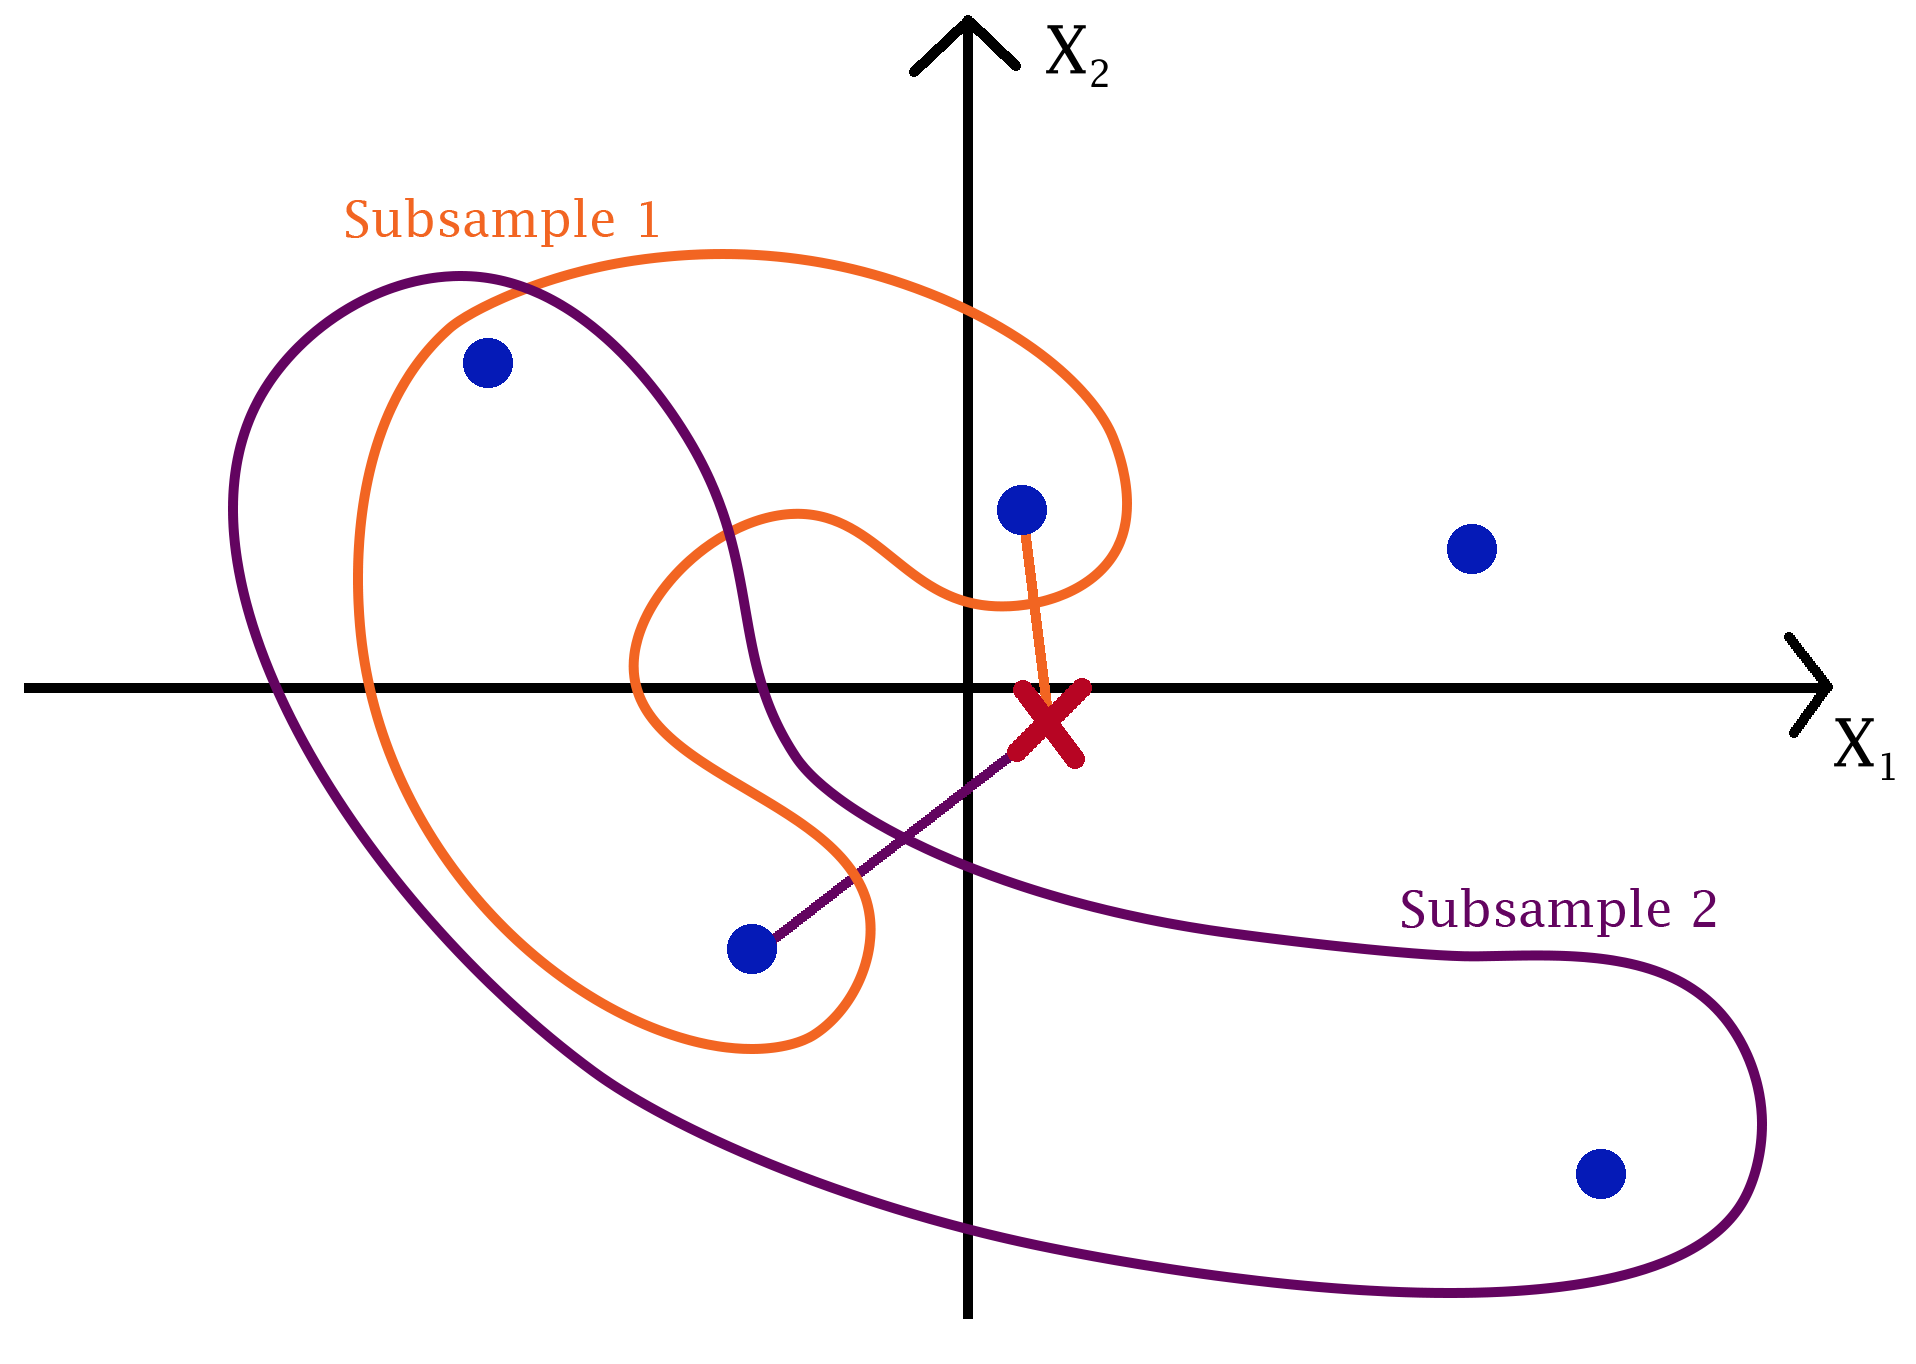
\includegraphics[width=0.8\linewidth]{Graphics/DNN_Estimator_Vis.png}
    \captionof{figure}{Visualization of the DNN Kernel Function}
\end{minipage}

Using $\kappa$, it is straightforward to find an expression for the distance function $K$ in Equation~\ref{EmpCondMomEq} corresponding to the DNN estimator.
\begin{equation}\label{eq:data_distance}
	K(x, X_{i})
	= \binom{n}{s}^{-1} \sum_{\ell \in L_{n,s}} \1(i \in \ell)\frac{\kappa(x; Z_{i}, D_{\ell})}{s!}
	= \binom{n}{s}^{-1} \sum_{\ell \in L_{n,s}} \frac{\1\left(\rk(x; Z_{i}, D_{\ell}) = 1\right)}{s!}
\end{equation}
Inserting into Equation~\ref{EmpCondMomEq}, this gives us the following empirical conditional moment equation.
\begin{equation}
	\begin{aligned}
		M_n(x; \mu, \mathbf{D}_n)
		= \sum_{i = 1}^{n}\left(\binom{n}{s}^{-1} \sum_{\ell \in L_{n,s}} \frac{\1\left(\rk(x; Z_{i}, D_{\ell}) = 1\right)}{s!}\right)\left(Y_{i} - \mu(X_{i})\right)
		= 0
	\end{aligned}
\end{equation}
Solving this empirical conditional moment equation then yields the DNN estimator $\tilde{\mu}_{s}(x)$ with subsampling scale $s$.
Defining the kernel function, $h_{s}(x; D_{\ell}) := (s!)^{-1} Y_{(1)}(x; D_{\ell})$, it is given by the following U-statistic.
\begin{equation}\label{eq:U_stat}
	\tilde{\mu}_{s}(x; \mathbf{D}_n)
	= \binom{n}{s}^{-1} \sum_{\ell \in L_{n,s}} h_{s}(x; D_{\ell})
\end{equation}
\citet{steele_exact_2009} shows that the DNN estimator has a simple closed form representation based on the original ordered sample.
\begin{equation}\label{eq:DNN_closed_form}
	\tilde{\mu}_{s}(x; \mathbf{D}_n)
	= \binom{n}{s}^{-1} \sum_{i = 1}^{n - s + 1}\binom{n - i}{s - 1}Y_{(i)}
\end{equation}
This representation will allow me to derive computationally simple representations for the practical use of the procedures presented in this paper.
This is in contrast to most U-statistic based methods that inherently rely on evaluating the kernel on individual subsets, incurring a potentially prohibitive computational cost.
Furthermore, this representation motivates an asymptotic approximation of the weights assigned to each observation that starkly reduces the potentially computationally intensive computation of large binomial coefficients.
For this purpose let $\alpha_{s} = s/n$ leading to the following approximation of the DNN estimator using asymptotic weights.
\begin{equation}\label{eq:DNN_approx_closed_form}
	\tilde{\mu}_{s}(x; \mathbf{D}_n)
	\approx  \sum_{i = 1}^{n - s + 1} \alpha_{s} \left(1 - \alpha_{s}\right)^{i - 1} Y_{(i)}
\end{equation}
It is worthwhile to point out that the role of $s$ in the implicit bias-variance trade-off of the DNN estimator runs counter to the role of $k$ in the usual k-NN regression.
Where a larger $k$ is usually associated with a lower variance at the cost of a higher bias, a larger $s$ does the opposite.
This is due to the fact that a higher $s$ reduces the number of observations that can occur as the closest observation in any given $s$-subset.
As a special example that illustrates the relationship, consider the DNN estimator choosing $s = n$ recovering the simple 1-NN regression estimator.
As part of their paper, \citet{demirkaya_optimal_2024} develop an explicit expression for the first-order bias term of the DNN estimator and the following distributional approximation result.
\begin{boxD}
	\begin{thm}[\citet{demirkaya_optimal_2024} - Theorem 2]\label{thm:dem2}\mbox{}\\*
		Assume that we observe data as described in Assumption~\ref{asm:npr_dgp} and that Assumption~\ref{asm:technical} is valid.
		Then, for any fixed $x \in \mathcal{X}$, we have for some positive sequence $\omega_n$ of order $\sqrt{s/n}$
		\begin{equation}
			\frac{\tilde{\mu}_{s}(x; \mathbf{D}_n) - \mu(x) - B(s) - R(s)}{\omega_n}
			\rightsquigarrow \mathcal{N}\left(0,1\right)
		\end{equation}
		as $n,s \rightarrow \infty$ with $s = o(n)$.
		Here, $B(s)$ and $R(s)$ are defined as the following bias terms.
		\begin{align}
			B(s)
			= \Gamma(2 / k+1) \frac{f(x) \operatorname{tr}\left(\mu^{\prime \prime}(x)\right)+2 \mu^{\prime}(x)^T f^{\prime}(x)}{2 d V_d^{2 / k} f(x)^{1+2 / k}} s^{-2 / k}
			\quad \text{and} \quad
			R(s) =
			\begin{cases}
				O\left(s^{-3}\right),     & k = 1      \\
				O\left(s^{-4 / k}\right), & k \geq 2
			\end{cases}
		\end{align}
		where\dots
		\begin{multicols}{2}
			\begin{itemize}
				\item $V_d=\frac{k^{k / 2}}{\Gamma(1+k / 2)}$
				\item $\Gamma(\cdot)$ is the gamma function
				\item $\operatorname{tr}(\cdot)$ stands for the trace of a matrix
				\item $f^{\prime}(\cdot)$ and $\mu^{\prime}(\cdot)$ denote the first-order gradients of $f(\cdot)$ and $\mu(\cdot)$, respectively
				\item $f^{\prime \prime}(\cdot)$ and $\mu^{\prime \prime}(\cdot)$ represent the $d \times d$ Hessian matrices of $f(\cdot)$ and $\mu(\cdot)$, respectively
			\end{itemize}
		\end{multicols}
	\end{thm}
\end{boxD}

Starting from this set-up, \citet{demirkaya_optimal_2024} develop a novel bias correction method for the DNN estimator that leads to appealing finite-sample properties of the resulting Two-Scale Distributional Nearest Neighbor (TDNN) estimator. 
Their method is based on the explicit formula for the first-order bias term of the DNN estimator, which in turn allows them to eliminate it through a clever combination of two DNN estimators. 
Choosing two subsampling scales $1 \leq s_1 < s_2 \leq n$ and two corresponding weights
\begin{equation}
	w_{1}^{*}(s_1, s_2) = \frac{1}{1-(s_1/s_2)^{-2/k}}
	\quad\text{and}\quad
	w_2^{*}(s_1, s_2) = 1 - w_{1}^{*}(s_1, s_2)
\end{equation}
they define the corresponding TDNN estimator as follows.
\begin{equation}
	\hat{\mu}_{s_1, s_2}\left(x; \mathbf{D}_n\right)
	= w_{1}^{*}(s_1, s_2)\tilde{\mu}_{s_1}\left(x; \mathbf{D}_n\right) + w_2^{*}(s_1, s_2)\tilde{\mu}_{s_2}\left(x; \mathbf{D}_n\right)
\end{equation}
This leads to the elimination of the first-order bias term shown in Theorem~\ref{thm:dem2} leading to desirable finite-sample properties.
Furthermore, the authors show that this construction improves the quality of the normal approximation.

\begin{boxD}
	\begin{asm}[Bounded Ratio of Kernel-Orders]\label{asm:kernel_order_ratio}\mbox{}\\*
		There is a constant $\mathfrak{c} \in (0,1/2)$ such that the ratio of kernel orders is bounded in the following way.
		\begin{equation}
			\forall n: \quad 0 < \mathfrak{c} \leq s_1 / s_2 \leq 1 - \mathfrak{c} < 1.
		\end{equation}
	\end{asm}
\end{boxD}
We make this assumption to avoid edge cases, where asymptotically the TDNN estimator converges to one of the DNN estimators that make it up.
As this edge case is irrelevant in practice and as it would be simpler to employ the corresponding DNN estimator in the first place, this is not a practically substantial restriction.
\begin{boxD}
	\begin{thm}[\citet{demirkaya_optimal_2024} - Theorem 3]\label{thm:dem3}\mbox{}\\*
		Assume that we observe data as described in Assumption~\ref{asm:npr_dgp} and that Assumption~\ref{asm:technical} holds.
		Furthermore, let $s_1, s_2 \rightarrow \infty$ with $s_1 = o(n)$ and $s_2 = o(n)$ be such that Assumption~\ref{asm:kernel_order_ratio} holds for some $\mathfrak{c} \in (0, 1/2)$.
		Then, for any fixed $x \in \operatorname{supp}(X) \subset \mathbb{R}^d$, it holds that for some positive sequence $\sigma_n$ of order $(s_2/n)^{1/2}$,
		\begin{equation}
			\sigma_n^{-1} \left(\hat{\mu}_{s_1, s_2}\left(x; \mathbf{D}_n\right) - \mu(x) - \Lambda\right) \rightsquigarrow \mathcal{N}(0,1)
		\end{equation}
		as $n \rightarrow \infty$, where
		\begin{equation*}
			\Lambda = \begin{cases}
				O\left(s_1^{-4/d} + s_2^{-4/d}\right) & \text{for } d \geq 2 \\
				O\left(s_1^{-3} + s_2^{-3}\right)     & \text{for } d = 1    \\
			\end{cases} .
		\end{equation*}
	\end{thm}
\end{boxD}
As most of the theoretical results in this paper rely on representing the estimators as a U-statistics, it is helpful to introduce additional concepts and notation at this stage.
Recalling Equation~\ref{eq:U_stat}, the DNN and TDNN estimators can be expressed in the following U-statistic form and are thus a type of generalized complete U-statistic as introduced by \citet{peng_rates_2022}.
\begin{equation}
	\tilde{\mu}_{s}(x; \mathbf{D}_n)
	= \binom{n}{s}^{-1} \sum_{\ell \in L_{n,s}} h_{s}(x; \mathbf{D}_{\ell})
	\quad \text{and} \quad
	\hat{\mu}_{s_1, s_2}(x; \mathbf{D}_n)
	= \binom{n}{s}^{-1} \sum_{\ell \in L_{n,s_2}} h_{s_1, s_2}(x; \mathbf{D}_{\ell})
\end{equation}
It is worth pointing out that in contrast to the DNN estimator, the kernel for the TDNN estimator is of order $s_2 > s_1$.
The authors derive an explicit formula for the kernel that shows the connection between the DNN and TDNN estimators.
This connection will prove useful going forward.
\begin{boxD}
	\begin{lem}[Kernel of TDNN Estimator - Adapted from Lemma 8 of \citet{demirkaya_optimal_2024}]\label{lem:dem8}\mbox{}\\*
		The kernel of the TDNN estimator takes the following form.
		\begin{equation}
			\begin{aligned}
				h_{s_1, s_2}\left(x; D\right)
				 & = w_{1}^{*}\left[\binom{s_2}{s_1}^{-1}\sum_{\ell \in L_{s_2, s_1}} h_{s_1}\left(x; \mathbf{D}_{\ell}\right)\right] + w_{2}^{*} h_{s_2}\left(x; D\right) \\
				 & = w_{1}^{*} \tilde{\mu}_{s_1}\left(x; D\right) + w_{2}^{*} h_{s_2}\left(x; D\right)                                                            \\
			\end{aligned}
		\end{equation}
	\end{lem}
\end{boxD}
Borrowing the notational conventions from \citet{lee_u-statistics_2019}, I furthermore introduce the following definitions for the purposes of studying the Hoeffding decompositions of the estimators of interest.
\begin{equation}\label{eq:psi_s_c}
	\psi_{s}^{c}(x; \mathbf{z}_{1}, \dotsc, \mathbf{z}_{c})
	= \E_{D}\left[h_{s}\left(x; D\right) \, | \,  Z_1 = \mathbf{z}_{1}, \dotsc, Z_c = \mathbf{z}_{c}\right]
\end{equation}
\begin{equation}
	h_{s}^{(1)}\left(x; \mathbf{z}_{1}\right)
	= \psi_{s}^{1}(x; \mathbf{z}_{1}) - \mu(x)
\end{equation}
\begin{equation}
	h_{s}^{(c)}\left(x; \mathbf{z}_{1}, \dotsc, \mathbf{z}_{c}\right)
	= \psi_{s}^{c}(x; \mathbf{z}_{1}, \dotsc, \mathbf{z}_{c}) - \sum_{j = 1}^{c-1}\left(\sum_{\ell \in L_{c,j}}h_{s}^{(j)}(x; \mathbf{z}_{\ell})\right) - \mu(x)
	\quad \text{for } c = 2, \dotsc, s
\end{equation}
In contrast to the notational inspiration, the subsampling size $s$ is made explicit.
Since we are dealing with an infinite-order U-statistic, $s$ will be diverging with $n$.
Completely analogous, define the corresponding objects for the TDNN estimator.
The main purpose of this additional notation is to derive the Hoeffding decomposition of the TDNN estimator.
\begin{equation}\label{eq:H_projection}
	\begin{aligned}
		H_{s}^{c}\left(x; \mathbf{D}_n\right)
		= \binom{n}{c}^{-1} \sum_{\ell \in L_{n,c}} h^{(c)}_{s}(x; \mathbf{D}_{\ell})
		\quad \text{and} \quad
		H_{s_1, s_2}^{c}\left(x; \mathbf{D}_n\right)
		= \binom{n}{c}^{-1} \sum_{\ell \in L_{n,c}} h^{(c)}_{s_1, s_2}(x; \mathbf{D}_{\ell})
	\end{aligned}
\end{equation}
These projection terms can then be used to construct the following Hoeffding decompositions.
\begin{equation}\label{eq:H_Decomp}
	\tilde{\mu}_{s}\left(x; \mathbf{D}_n\right)
	= \mu(x) + \sum_{j = 1}^{s}\binom{s}{j}H_{s}^{j}\left(x; \mathbf{D}_n\right)\\
	\quad \text{and} \quad
	\hat{\mu}_{s_1, s_2}\left(x; \mathbf{D}_n\right)
	= \mu(x) + \sum_{j = 1}^{s_2}\binom{s_2}{j}H_{s_1, s_2}^{j}\left(x; \mathbf{D}_n\right)
\end{equation}

\subsection{DNN in CATE Estimation}
\hrule
Motivated by the nonparametric regression setup, I set out to apply the underlying idea in the context of heterogeneous treatment effects.
Similarly to before, I start by specifying a moment corresponding to our object of interest, taking into account the additional factors that come into play.
Due to the presence of a high-dimensional nuisance parameter in the form of the function $q$, it is natural to apply the concepts of DDML.
This approach closely follows the leading example of \citet{ritzwoller_simultaneous_2024}.
The main goal at this stage is to construct a highly practical method based on their ideas that leverages the computational simplicity of the distributional nearest-neighbor framework.\\

While considering the problem of point-estimation of a conditional average
treatment effect given a feature vector $x$,
$\theta_{0}(x) = \E\left[Y_{i}\left(W_{i} = 1\right) -
		Y_{i}\left(W_{i} = 0\right) \, \middle| \, X_{i} = x\right]$, I
will employ a Neyman-orthogonal score function to curtail the influence of the
nuisance parameters on our estimation.
\begin{equation}
	\begin{aligned}
		M(x; \theta_{0}, \eta)
		 & = \E\left[m\left(Z_{i}; \theta, \eta\right) \, \middle| \, X_{i} = x\right]
		= 0
		\quad \text{where} \quad                                                                                                                                                                                       \\
		m\left(Z_{i}; \theta, \eta\right)
		 & = \mu^{1}\left(X_{i}\right) - \mu^{0}\left(X_{i}\right) + \beta\left(W_{i}, X_{i}\right)\left(Y_{i} - \mu^{W_{i}}\left(X_{i}\right)\right) - \theta\left(X_{i}\right)
	\end{aligned}
\end{equation}
Here, I make use of the following notation, that is common in the potential
outcomes framework, and the well-known Horvitz-Thompson weight.
\begin{equation}
	\text{for }  w = 1,2: \quad \mu_w\left(x\right) = \E\left[Y_{i} \, \middle| \, W_{i} = w, \; X_{i} = x\right]
	\quad \text{and} \quad
	\beta\left(w, x\right) = \frac{w}{\pi\left(x\right)} - \frac{1 - w}{1 - \pi\left(x\right)}
\end{equation}
As a shorthand notation, I will furthermore use $m\left(Z_{i}; \eta\right) = m\left(Z_{i}; \theta_{0}, \eta\right) + \theta_{0}\left(X_{i}\right)$.
This notation will mainly be used to shorten the presentation of proofs in the appendix.
Proceeding in an analogous fashion to the nonparametric regression setup leads us to the following empirical moment equation, where $\hat{\mu}$ and $\hat{\pi}$ are first-stage estimators and $K$ is the data-driven kernel function defined in Equation~\ref{eq:data_distance}.
\begin{equation}
	\begin{aligned}
		M_{n}\left(x; \hat{\eta}\right)
		= \sum_{i = 1}^{n} K(x, X_{i}) m\left(Z_{i}; \hat{\eta}\right)
		= 0
	\end{aligned}
\end{equation}
However, due to the presence of infinite-dimensional nuisance parameters, it becomes attractive to proceed using this weighted empirical moment equation embedded in the DML2 estimator of \citet{chernozhukov_doubledebiased_2018}.
Applying these ideas to the context of estimating the CATE has been previously explored, for example by \citet{semenova_debiased_2021}
For the sake of simplicity, I will assume that $m = n/K$, i.e.\ the desired number of observations in each fold, is an integer going forward.
\begin{boxD}
	\begin{dfn}{DNN-DML2 CATE-Estimator}\label{def:CATE_DNN_DML}\mbox{}\\*
		To estimate the Conditional Average Treatment Effect at a point of interest $x \in \mathcal{X}$, proceed as follows.
		\begin{enumerate}
			\item Take a $K$-fold random partition $\mathcal{I} = \left(I_k\right)_{k = 1}^{K}$
			      of the observation indices $[n]$ such that the size of each fold $I_k$ is $m =
				      n/K$. For each $k \in [K]$, define $I_{k}^{C} = [n] \backslash I_k$.
			      Furthermore, for the observation being assigned rank $i \in [n]$, denote by
			      $k_{(i)}$ the fold that the observation appears in.
                  In contrast, for observation $j$ (\textbf{NOT} the observation being assigned rank $j$) denote the corresponding fold by $k_j$.
			\item For each $k \in [K]$, use a first-stage estimator for the functional nuisance parameters on the data set
			      $\mathbf{D}_{I_k^C}$\dots
			      \begin{enumerate}
				      \item to estimate the nuisance parameters $\mu_{0}^{0}$ and $\mu_{0}^{1}$:
				            \begin{equation}
					            \hat{\mu}_{k}^{w}\left(x\right) = \hat{\mu}\left(x; \mathbf{D}_{I_k^{C}}^{(w)}\right) \quad \text{for } w=0,1
				            \end{equation}
				      \item if $\pi_{0}$ is unknown, i.e.\ we are not in a randomized experiment setting,
				            additionally estimate $\pi_{0}$
				            \begin{equation}
					            \hat{\pi}_{k}\left(x\right) = \hat{\mu}\left(x; \mathbf{D}_{I_k^{C}}\right) \quad \text{where the predicted variable is $W$}
				            \end{equation}
			      \end{enumerate}
            For each fold $k$, denote the vector of estimates by $\hat{\eta}_{k} = \left(\hat{\mu}_{k}^{0}, \hat{\mu}_{k}^{1}, \hat{\pi}_{k}\right)^{\prime}$.
            For each observation $i$, define the combined estimator as follows $\hat{\eta}(Z_i) = \hat{\eta}_{k_{i}}(Z_i)$.
			\item Construct the estimator $\hat{\theta}\left(x\right)$
			      as the solution to the following equation.
			      \begin{equation}
				      \begin{aligned}
					      0 = \sum_{k = 1}^{K} \sum_{i \in I_k} K(x, X_{i}) m\left(Z_{i}; \hat{\theta}\left(x\right), \hat{\eta}_{k}\right)
					      = \sum_{i = 1}^{n - s + 1} \frac{\binom{n-i}{s-1}}{\binom{n}{s}} m\left(Z_{(i)}; \hat{\theta}\left(x\right),\hat{\eta}_{k_{(i)}}\right)
				      \end{aligned}
			      \end{equation}
		\end{enumerate}
	\end{dfn}
\end{boxD}
Observe that the weights $K(x, X_{i})$ chosen in the second step are chosen according to the whole sample - not according to the chosen folds.
Using a lower choice of subsampling scale for this estimation step can help avoid extreme values in the Neyman-orthogonal score function due to estimated propensity scores close to zero or one.
This is because a lower subsampling scale averages over a larger number of observations and thus can contribute to better smoothing properties for the propensity score.
Using the score function in the equation that defines the estimator, we can observe the following.
\begin{equation}
	\begin{aligned}
		\hat{\theta}\left(x\right) 
        & = \sum_{i = 1}^{n - s + 1} \frac{\binom{n-i}{s-1}}{\binom{n}{s}} m(Z_{(i)}, \hat{\eta}_{k_{(i)}})
	\end{aligned}
\end{equation}

Thus, given first-stage estimates of nuisance parameters, I have a closed-form representation of the CATE estimator for a given partition of $[n]$.
Furthermore, given these first-stage estimates, the evaluation of the CATE-estimator at a different point of interest is merely a re-weighting of the terms corresponding to different observations.
As is typical in the literature on doubly-robust inference, we need to make assumptions on the convergence rate of the first-stage estimators to allow for the desired type of inference.
Specifically, I take the following slightly modified assumptions from Assumption 3.2 of \citet{chernozhukov_doubledebiased_2018}. 
\begin{boxD}
    \begin{asm}[DDML-Rate Conditions]\label{asm:DDML_Rate_Cond}\mbox{}\\*
        Let $\left\{\delta_n\right\}_{n \geq 1}$ and $\left\{\Delta_n\right\}_{n \geq 1}$ be some sequences of positive constants converging to zero such that $\delta_n \geq n^{-1 / 2}$. 
        \begin{enumerate}
            \item Given a random subset $I$ of $[n]$ of size $m = n/k$, the nuisance parameter estimator $\hat{\eta}\left(\mathbf{D}_{I^{C}}\right)$ belongs to the realization set $\mathcal{T}_{n}$ with probability $1 - \Delta_{n}$, where $\mathcal{T}_{n}$ contains $\eta_{0}$ and is constrained by the following conditions. 
            Denote the event that $\hat{\eta}\left(\mathbf{D}_{I^{C}}\right) \in \mathcal{T}_{n}$ by $\mathcal{E}_{n}$.
            \item The following moment condition holds:
            \begin{align}
                m_{n} 
                & :=\sup_{\eta \in \mathcal{T}_{n}}\left(\E_{Z}\left[\left|m\left(Z; \theta_0, \eta\right)\right|^q\right]\right)^{1 / q}
                \leq c_1
                % m_{n}^{\prime} 
                % & :=\sup_{\eta \in \mathcal{T}_{n}}\left(\E_{Z}\left[\left|\psi^a(Z; \eta)\right|^q\right]\right)^{1 / q} 
                % \leq c_1 .
            \end{align}
            \item The following conditions on the statistical rates $r_{n}$, $r_{n}^{\prime}$, and $\lambda_{n}^{\prime}$ hold:
            \begin{align}
                % r_{n}
                % & :=\sup_{\eta \in \mathcal{T}_{n}}\left|\E_{Z}\left[\psi^a(Z; \eta)\right]-\E_{Z}\left[\psi^a\left(Z; \eta_0\right)\right]\right| 
                % \leq \delta_{n}, \\
                % %
                r_{n}^{\prime}
                & :=\sup_{\eta \in \mathcal{T}_{n}}\left(\E_{Z}\left[\left|m\left(Z; \theta_0, \eta\right)-m\left(Z; \theta_0, \eta_0\right)\right|^2\right]\right)^{1 / 2} 
                \leq \delta_{n}, \\
                %
                \lambda_{n}^{\prime}
                & :=\sup_{r \in(0,1), \eta \in \mathcal{T}_{n}}\left|\partial_r^2 \E_{Z}\left[m\left(Z; \theta_0, \eta_0+r\left(\eta-\eta_0\right)\right)\right]\right| 
                \leq \delta_{n} / \sqrt{n} .
            \end{align}
            \item The variance of the score is non-zero.
            \begin{equation}
                \exists \mathfrak{v} \quad \text{such that} \quad 
                0 < \mathfrak{v} \leq \E_{Z}\left[m^{2}\left(Z; \theta_0, \eta_0\right)\right]
            \end{equation}
        \end{enumerate}
    \end{asm}    
\end{boxD}
In contrast to the paper that these assumptions are taken from, there is an absence of conditions on what is named $\psi^{a}$ in the original paper.   This is due to the fact that in the case of the CATE, this term is $-1$ and thus independent of the nuisance parameters.
Thus, specific constraints on the effects of the first-stage estimation problem are unnecessary.
In a potential generalization of the method proposed in this paper to other doubly-robust inference problems, this aspect should be addressable with relatively minimal additional technical arguments along the lines in \citet{chernozhukov_doubledebiased_2018}.

Given estimates of the functional nuisance parameters, the proposed CATE estimators can be analyzed as generalized U-statistics in the same way as in the nonparametric regression context.
As most of the theoretical results on these estimators will similarly rely on Hoeffding projection arguments, I will introduce analogous notation in this more general scenario.
First, observe that the DNN-DML2 CATE estimator can be rewritten as follows to explicitly show its construction as a generalized U-statistic.
\begin{equation}
    \begin{aligned}
        \hat{\theta}\left(x; \mathbf{D}\right) 
        & = \sum_{i = 1}^{n - s + 1} \frac{\binom{n-i}{s-1}}{\binom{n}{s}}
		\left[\hat{\mu}_{k_{(i)}}^{1}\left(X_{(i)}\right) - \hat{\mu}_{k_{(i)}}^{0}\left(X_{(i)}\right) + \hat{\beta}_{k_{(i)}}\left(W_{(i)}, X_{(i)}\right)\left(Y_{(i)} - \hat{\mu}^{W_{(i)}}_{k_{(i)}}\left(X_{(i)}\right)\right)\right] \\
        %
        & = \binom{n}{s}^{-1} \sum_{\ell \in L_{n,s}}
        \sum_{i = 1}^{n}\frac{\1\left(\rk(x; Z_{i}, \mathbf{D}_{\ell}) = 1\right)}{s!} 
        \left[\hat{\mu}_{k_i}^{1}\left(X_{i}\right) - \hat{\mu}_{k_i}^{0}\left(X_{i}\right) + \hat{\beta}_{k_i}\left(W_{i}, X_{i}\right)\left(Y_{i} - \hat{\mu}^{W_{i}}_{k_i}\left(X_{i}\right)\right)\right] \\
        %
        & = \binom{n}{s}^{-1} \sum_{\ell \in L_{n,s}}
        \underbrace{\sum_{i = 1}^{n}\frac{\1\left(\kappa(x; Z_{i}, \mathbf{D}_{\ell}) = 1\right)}{s!} 
        m(Z_{i}, \hat{\eta}_{k_i})}_{\chi_{s}(x; \mathbf{D}_{\ell}, \hat{\eta})}
        = \binom{n}{s}^{-1} \sum_{\ell \in L_{n,s}}\chi_{s}(x; \mathbf{D}_{\ell}, \hat{\eta})
    \end{aligned}
\end{equation}
To use arguments based on the Hoeffding-projection of this estimator, introduce the following additional notation.
\begin{alignat}{4}
    &\chi_{s, 0}(x; \mathbf{D}_{[s]})
    & \; := \; &\chi_{s}(x; \mathbf{D}_{[s]}, \eta_{0}),\\
    %
    &\vartheta_{s}^{c}\left(x; \mathbf{z}_{1}, \dotsc, \mathbf{z}_{c}, \eta\right)
    & \; := \; &\E_{D}\left[\chi_{s}(x; \mathbf{D}, \eta) \, \middle| \, Z_1 = \mathbf{z}_1, \dotsc, Z_c = \mathbf{z}_c\right], &
    \hspace{1cm}
    &\vartheta_{s,0}^{c}\left(x; \mathbf{z}_{1}, \dotsc, \mathbf{z}_{c}\right)
    & \; := \; &\vartheta_{s}^{c}\left(x; \mathbf{z}_{1}, \dotsc, \mathbf{z}_{c}, \eta_{0}\right), \\
    %
    &\chi_{s}^{(1)}\left(x; \mathbf{z}_{1}, \eta\right)
	& \; := \; &\vartheta_{s}^{1}\left(x; \mathbf{z}_{1}, \eta\right)
    - \E_{D}\left[\chi_{s}(x; \mathbf{D}, \eta)\right], &
    \hspace{1cm}
    &\chi_{s,0}^{(1)}\left(x; \mathbf{z}_{1}\right)
	& \; := \; &\chi_{s}^{(1)}\left(x; \mathbf{z}_{1}, \eta_{0}\right)
\end{alignat}
% As before, I define the higher-order projection terms, i.e. for $c = 2, \dotsc, s$, in the following way.
% \begin{equation}
%     \chi_{s}^{(c)}\left(x; \mathbf{z}_{1}, \dotsc, \mathbf{z}_{c}, \eta\right)
% 	= \vartheta_{s}^{c}(x; \mathbf{z}_{1}, \dotsc, \mathbf{z}_{c}, \eta) 
%     - \sum_{j = 1}^{c-1}\left(\sum_{\ell \in L_{c,j}} \chi_{s}^{(j)}(x; \mathbf{z}_{\ell}, \eta)\right) 
%     - \E_{D}\left[\chi_{s}(x; \mathbf{D}, \eta)\right]
% \end{equation}
% \begin{equation}
%     \begin{aligned}
%         \chi_{s,0}^{(c)}\left(x; \mathbf{z}_{1}, \dotsc, \mathbf{z}_{c}\right)
% 	    & = \chi_{s}^{(c)}\left(x; \mathbf{z}_{1}, \dotsc, \mathbf{z}_{c}, \eta_{0}\right) \\
%         %
%         & = \vartheta_{s,0}^{c}(x; \mathbf{z}_{1}, \dotsc, \mathbf{z}_{c}) 
%         - \sum_{j = 1}^{c-1}\left(\sum_{\ell \in L_{c,j}} \chi_{s,0}^{(j)}(x; \mathbf{z}_{\ell})\right) 
%         - \E_{D}\left[\chi_{s,0}\left(x; Z_{1}, \dotsc, Z_{c}\right)\right]
%     \end{aligned}
% \end{equation}
% These definitions allow us to use the following decomposition.
% \begin{equation}\label{eq:DNNDML2_ResidDecomp}
%     \begin{aligned}
%         \chi_{s}^{(c)}\left(x; \mathbf{D}_{\ell}, \eta\right)
%         & = \chi_{s,0}^{(c)}\left(x; \mathbf{D}_{\ell}\right) + \underbrace{\chi_{s}^{(c)}\left(x; \mathbf{D}_{\ell}, \eta\right) - \chi_{s,0}^{(c)}\left(x; \mathbf{D}_{\ell}\right)}_{R_{c}\left(x; \mathbf{D}_{\ell}, \eta\right)}
%     \end{aligned}
% \end{equation}
% Considering this decomposition will be of great usefulness when analyzing the asymptotic properties of the CATE estimators.
% Let $\hat{\mu}_{k}$ and $\hat{\pi}_{k}$ denote the nuisance parameter estimates calculated on the complement of fold $k$.
Using the full expression for the CATE estimator, we obtain the following crucial representation of the estimator.
\begin{equation}\label{eq:DNNDML2_Decomp}
    \begin{aligned}
        \hat{\theta}\left(x; \mathbf{D}\right)
        & = \underbrace{\underbrace{\E_{D}\left[\hat{\theta}_{0}\left(x; \mathbf{D}\right)\right]}_{\text{Centering-Term}}
        + \underbrace{\frac{s}{n}\sum_{i = 1}^{n} \chi_{s,0}^{(1)}\left(x; Z_{i}\right)}_{\text{Oracle-H\'ajek-Projection}}
        + \underbrace{\sum_{j = 2}^{s} \binom{s}{j} \binom{n}{j}^{-1}\sum_{\ell \in L_{n,j}} \chi_{s,0}^{(j)}\left(x; \mathbf{D}_{\ell}\right)}_{\text{Oracle-H\'ajek-Residual}}}_{\text{Oracle-Hoeffding-Projection}}\\
        & \quad \quad + \underbrace{\binom{n}{s}^{-1}\sum_{\ell \in L_{n,s}}\left(\chi_{s}\left(x; \mathbf{D}_{\ell}, \hat{\eta}\right) - \chi_{s,0}\left(x; \mathbf{D}_{\ell}\right)\right)}_{\text{First-Stage Approximation Error}}
    \end{aligned}
\end{equation}

\subsection{Asymptotic Normality of the DNN-DML2 CATE Estimator}\label{CATE_AsympNorm}
\hrule

As a first intermediate result in the analysis of the asymptotic properties of the CATE estimator, we can find the following concerning an oracle variant of the proposed estimator defined as the solution to the following problem.
\begin{equation}\label{eq:DNNDML2_Oracle}
    \begin{aligned}
        0 
        = \sum_{i = 1}^{n} K(x, X_{i}) m\left(Z_{i}; \hat{\theta}_{0}(x), \eta_{0}\right)
        = \sum_{i = 1}^{n - s + 1} \frac{\binom{n-i}{s-1}}{\binom{n}{s}} m\left(Z_{(i)}; \hat{\theta}_{0}(x),\eta_{0}\right)
    \end{aligned}
\end{equation}
This is a rather basic result that can be seen as a corollary to the nonparametric regression case.
\begin{boxD}
	\begin{thm}[Asymptotic Normality of the Oracle-DNN-DML2 CATE Estimator]\label{thm:DNNDML2_anorm_0}\mbox{}\\*
		Assume that we observe a data set $\mathbf{D}_{[n]}$ as described in Assumption~\ref{asm:CATE_dgp}. 
        Furthermore, assume that Assumptions \ref{asm:technical}, \ref{asm:errors}, and \ref{asm:treatment_overlap} are valid.
		Then, for any fixed $x \in \mathcal{X}$, we have for some positive sequence $\omega_{n,0}$ of order $\sqrt{s/n}$
		\begin{equation}
			\frac{\hat{\theta}_{0}(x; \mathbf{D}_{[n]}) - \theta_{0}(x)}{\omega_{n,0}}
			\rightsquigarrow \mathcal{N}\left(0,1\right)
		\end{equation}
		as $n,s \rightarrow \infty$ with $s = o(n)$.
	\end{thm}
\end{boxD}
More important is the following result showing asymptotic normality of the full estimator using cross-fitted first-stage estimates for the functional nuisance parameters.
\begin{boxD}
	\begin{thm}[Asymptotic Normality of the DNN-DML2 CATE Estimator]\label{thm:DNNDML2_anorm}\mbox{}\\*
		Assume that we observe a data set $\mathbf{D}_{[n]}$ as described in Assumption~\ref{asm:CATE_dgp}.
        Furthermore, assume that Assumptions \ref{asm:technical}, \ref{asm:errors}, \ref{asm:treatment_overlap}, and \ref{asm:DDML_Rate_Cond} are valid.
		Then, for any fixed $x \in \mathcal{X}$, we have for some positive sequence $\omega_n$ of order $\sqrt{s/n}$
		\begin{equation}
			\frac{\hat{\theta}(x; \mathbf{D}_{[n]}) - \theta_{0}(x)}{\omega_n}
			\rightsquigarrow \mathcal{N}\left(0,1\right)
		\end{equation}
		as $n,s \rightarrow \infty$ with $s = o\left(\min\left\{1/r_{n}^{\prime}, \left(\sqrt{n} \cdot \lambda_{n}^{\prime}\right)^{-1}\right\}\right)$ with rates corresponding to Assumption \ref{asm:DDML_Rate_Cond}.
	\end{thm}
\end{boxD}
{\color{red} LOREM IPSUM}

